\documentclass[a4paper,abstract=true]{scrartcl}

% ----- Encoding & Fonts
\usepackage[T1]{fontenc}
\usepackage[utf8]{inputenc}
\usepackage{lmodern}
\usepackage{microtype}


\usepackage[english, ngerman]{babel}

% ----- Zitate/Anführungen
\usepackage{csquotes}

% ----- Grafik & Layout
\usepackage{graphicx}
\usepackage{subcaption}
\usepackage{booktabs}
\usepackage{longtable}
\usepackage{tabularx,ragged2e}
\newcolumntype{Y}{>{\RaggedRight\arraybackslash}X}

% ----- URL/Links
\usepackage[hyphens,spaces,obeyspaces]{url}
\usepackage[hidelinks]{hyperref}
\usepackage{orcidlink}

\usepackage{cleveref}

% ----- biblatex (nach babel, csquotes, hyperref)
\usepackage[backend=biber,style=acmnumeric,doi=true,url=true]{biblatex}
\addbibresource{helios_prototype.bib}




% ----- Boxen, Listings etc.
\usepackage[most]{tcolorbox}
\newtcolorbox{summarybox}{
    enhanced, breakable, sharp corners,
    boxrule=0.3pt, colback=white, colframe=black!40,
    coltitle=black, fonttitle=\bfseries,
    toptitle=2mm, bottomtitle=2mm, colbacktitle=white,
}
\usepackage{listings}
\usepackage{xcolor}
\definecolor{codegray}{gray}{0.9}
\definecolor{commentgreen}{rgb}{0,0.6,0}
\definecolor{keywordblue}{rgb}{0.2,0.2,0.8}

\lstdefinestyle{c++style}{
    backgroundcolor=\color{white},
    commentstyle=\color{commentgreen}\itshape,
    keywordstyle=\color{keywordblue}\bfseries,
    numberstyle=\tiny\color{gray},
    stringstyle=\color{red},
    basicstyle=\ttfamily\small,
    breaklines=true,
    captionpos=b,
    keepspaces=true,
    numbers=left,
    numbersep=5pt,
    showspaces=false, showstringspaces=false, showtabs=false,
    tabsize=2, language=C++
}

% ----- Anhang
% Entweder KOMA intern nutzen (empfohlen) ODER appendix-Paket.
% Wenn du das Paket behalten willst, okay:
\usepackage[titletoc,title,page,header]{appendix}
\renewcommand{\appendixname}{Anhang}
\renewcommand{\appendixtocname}{Anhänge}
\renewcommand{\appendixpagename}{Anhänge}

% ----- Sonstiges
\usepackage{dirtree}
\renewcommand*\DTstyle{\ttfamily}

% Silbentrennungen
\hyphenation{
    Ren-de-ring-Back-end
    Game-Loop
    Smart-Poin-ter
    Kol-li-sions-be-hand-lung
    er-strek-ken
}


\begin{document}


    \title{helios: Konzeption und prototypische Umsetzung eines C++ Game Frameworks}

    \author{
        Thorsten Suckow-Homberg\,\orcidlink{0009-0002-3389-8606}\thanks{Trier University of Applied Sciences, Fachbereich Informatik, \email{thorsten@suckow-homberg.de}}
    }



    \maketitle




    \begin{abstract}
    Wir stellen \textit{helios} vor, einen in C++ entwickelten Prototyp eines Game Frameworks zur Umsetzung eines \textit{Geometry Wars}-Klons.
    Wir beschreiben den grundlegenden Aufbau des Frameworks und gehen auf die Funktionalitäten vorhandener Module ein.
    Architektur- und Designentscheidungen werden begründet, ebenso die Herausforderungen, die sich während der Entwicklung ergeben haben.
    Abschließend geben wir einen Ausblick, in welchen Bereichen wir im weiteren Verlauf der Entwicklung die größten Änderungen erwarten.
\end{abstract}

\section{Einleitung}

Zur Programmierung eines Spiel, das dem Shooter \textit{Geometry Wars}\footnote{siehe~\cite[]{WikipediaGeometryWars}} ähnelt, orientieren wir uns bei der Umsetzung des technischen Fundaments teilweise an einer in der Industrie weit verbreiteten, von \textit{Gregory} in~\cite[]{Gre19} beschriebenen \textit{Game Engine Architektur}, reduzieren jedoch bewusst die Anzahl der Abstraktionsschichten und verzichten auf Systeme wie Tooling, Sound oder Scripting (vgl.~\cite[\textbf{Figure 1.16}, 39]{Gre19}).
Damit entspricht die \textit{Hard Architecture}~\cite[]{RM04} einem Framework, welches Schnittstellen für benötigte Hardware und andere Subsysteme bereitstellt.
Das eigentliche Spiel kann die Schnittstellen des Frameworks nutzen, wird von diesem aber als \textit{Black Box}~\cite[]{RB88} betrachtet.\\

\begin{figure}[!h]
    \centering
    \includegraphics[width=1\columnwidth]{img/geometry_wars}
    \caption{Geometry Wars fand sich erstmals 2003 als Easter Egg in dem Spiel \textit{Project Gotham Racing} (Microsoft Game Studios). Aufgrund der großen Beliebtheit entstanden mehrere Nachfolger, zuletzt 2016 mit \textit{Geometry Wars 3: Dimensions Evolved} (Activision). (Quelle: Steam)}
    \label{fig:geometry_wars}
\end{figure}

In den nachfolgenden Abschnitten wird die Architektur von dem mit \textbf{helios}\footnote{
    Helios, der ``scharf vor allen mit strahlenden Augen umherblickt`` (\textit{Homers Ilias}, 14. Gesang), ist in der griechischen Mythologie der Sonnengott.
} getauften Framework vorgestellt.
Dabei berücksichtigen wir, dass es sich um einen in der Entwicklung befindlichen Prototypen handelt:
Die Software wird im Rahmen eines agilen \textit{Tracer Bullet Development}-Prozess~\cite[50 f.]{TH20} entwickelt.
Dadurch soll das Gesamtsystem verhältnis- und zweckmäßig angepasst werden können, woraus sich auch Anforderungen an die Architektur ableiten lassen.
In Abschnitt~\ref{sec:projektdaten} wird noch einmal gesondert auf die Anforderungen eingegangen. \\

\begin{figure}[!h]
    \centering
    \includegraphics[width=0.5\columnwidth]{img/helios_logo}
    \caption{Das helios Projekt-Logo.}
    \label{fig:helios_logo}
\end{figure}


Wir betrachten auch Probleme und Schwierigkeiten, die bei der bisherigen Umsetzung aufgetaucht sind.
Diese ergeben sich u.a. durch den Umstand, dass das in vergleichsweise kurzer Zeit zu erstellende Softwareprodukt nicht nur anhand \textit{objektiver} Maße bewertet werden soll (etwa der Fehleranzahl, Software-Designentscheidungen, Kopplungsgrad der Objekte etc.), sondern auch anhand \textit{subjektiver} Maße~\cite[385]{Bal08}.\\
Zwar ist keine Klassifizierung des fertigen Produkts nach Nutzungsqualitätsmerkmalen wie bspw. ISO/IEC 9126 angedacht\footnote{bspw. ``Nutzungsqualität nach ISO/IEC 9126``,~\cite[466]{Bal08}; Studien und Untersuchungen u.a. bei~\cite[]{AZMK17},~\cite[]{Ber10}}.
Dennoch soll das Ergebnis nicht nur technisch ausgereift sein, sondern auch für den Anwender angenehm zu bedienen.
Dieses Nutzererlebnis wird im Weiteren formal eher unscharf, aber mit dem in der Spieleentwicklung etablierten Begriff des \textit{Game Feel}~\cite[]{Swi08} zusammengefasst: Einem möglichst \textit{angenehmen} und in jeglicher Hinsicht \textit{positiven Spielerlebnis}.


\section{Projektziele und -daten}\label{sec:projektdaten}

Das Ziel der Projektarbeit ist es, einen stabil laufenden Prototyp des Twin-Stick Shooters\footnote{
Zur Genreeinteilung siehe auch \cite[]{GameDeveloper}
} \textit{Geometry Wars} (siehe Abbildung~\ref{fig:geometry_wars}) unter Verwendung der Programmiersprache \textit{C++} (23) und der OpenGL-API\footnote{siehe~\cite[]{OpenGLHomepage}
}  zu erstellen.\\

\noindent
Als grundsätzlich fertigzustellende Kernfeatures wurden vereinbart (siehe Anhang~\ref{sec:projektvorschlag}):

\vspace{2mm}
\begin{itemize}
    \itemsep0.5em
    \item Spielbares Level (2D-Grid)
    \item Time-Attack Modus mit einer Dauer von 3 Minuten
    \item Highscore-System
    \item Controller-Steuerung
    \item Stabile Framerate von mindestens 60 FPS bei gleichzeitiger Darstellung von über hundert Gegnern und Objekten
    \item Drei Gegnertypen mit einfacher KI (``Spawn and Chase``)
    \item Aufwertung des Game Feels durch grafische Effekte
    \item Compilierbar und lauffähig unter Windows 11
\end{itemize}
\vspace{2mm}

Während einige Kriterien konkret messbar sind (Framerate), sind andere Anforderungen bewusst unscharf formuliert (Game Feel) und unterstreichen den explorativen Charakter des Projekts.
Ein Requirements Engineering ist folglich auch nicht Bestandteil der Arbeit.
Als ein Maß dient neben den o.a. Kriterien vor allem auch das Original-Spiel, an dem sich die Umsetzung orientiert.\par

Der Lernprozess wird im Besonderen als ein wesentliches Ziel dieser Arbeit betrachtet, für dessen Bewertung keine formalen Metriken herangezogen werden.
Stattdessen sollen die gewonnenen Erfahrungen und Ergebnisse im Anschluss schriftlich festgehalten und das hier vorliegende Dokument kritisch reflektiert werden.\par

Vor diesem Hintergrund wird das Vorgehen als eine Form des dynamischen Requirements Engineering ``mit deutlich größeren Freiheitsgeraden``~\cite[60]{MRP21} betrachtet: Das erwähnte \textit{Tracer Bullet Development}, das vor allem eine Plattform zur Integration bereitstellt, entspricht dem von \textit{Pflug et al.} mit ``Living Lab`` bezeichneten Prototyp, der im Weiteren nach agilen Methoden entwickelt wird (\textit{ebd., S. 61})\footnote{
    Kasurinen et al. gehen in~\cite[]{KMS14} der Frage nach, ob das im Ingenieursbereich angesiedelte Anforderungsmanagement bei der stark durch kreative Prozesse beeinflussten Spieleentwicklung einen Platz hat. Sie zeigen, dass befragte Entwickler einen Teil der Anforderungen an ihr Spiel ganz bewusst erst durch \textit{User Testing} ableiten. Entsprechend stellt \textit{Games User Research} einen wichtigen Zweig der Spieleindustrie dar, der Unternehmen dabei unterstützt, Spiele-Erfahrung zu verstehen und zu verbessern (vgl.~\cite[26]{Zam18}). Weitere Diskussionen bzgl. Herausforderungen beim Software Engineering bei der Spielentwicklung in~\cite[]{KH09}.
}, und ein Einbringen eigener kreativer Ideen erlauben soll.\\

\subsection{Zeitplan}

Wir stellen den Zeitplan und die zugehörigen Meilensteine vor.
Die in Tabelle~\ref{tab:zeitplan} angegebene zeitliche Gliederung dient der Orientierung zur Umsetzung; die sequentielle Auflistung impliziert kein Wasserfallmodell.

\setlength{\tabcolsep}{8pt}
\begin{table}[t]
    \centering
    {\renewcommand{\arraystretch}{1.2}%
    \begin{tabularx}{\textwidth}{@{} l l Y @{}}
        \toprule
        \textbf{Meilenstein} & \textbf{Datum} & \textbf{Inhalt} \\
        \midrule
        \texttt{milestone\_1} & 20.10.2025 &
        Bereitstellung der Applikationsschicht inkl. Implementierung des Event-Systems,
        des Input-Managers sowie Anbindung an das Low-Level-API-Subsystem. \\
        \texttt{milestone\_2} & 17.11.2025 &
        Bereitstellung der Rendering-Engine; erster Entwurf des Spielfelds samt Darstellung des Spielerschiffs. \\
        \texttt{milestone\_3} & 22.12.2025 &
        Umsetzung der Physik und Spielereingabe zur Steuerung des Schiffs; Feuermechaniken. \\
        \texttt{milestone\_4} & 19.01.2026 &
        Implementierung der wichtigsten Spielregeln und -mechaniken; spielfähiger Prototyp. \\
        \texttt{milestone\_5} & 09.02.2026 &
        Bereitstellung des Prototyps; Feinschliff. \\
        \texttt{milestone\_6} & 16.03.2026 &
        Abgabe der Dokumentation und Vorstellung des Projekts. \\
        \bottomrule
    \end{tabularx}}
    \caption{Geplante Meilensteine zur Umsetzung des Geometry Wars Klon.}
    \label{tab:zeitplan}
\end{table}



\noindent
Mit der Vorgabe des umzusetzenden Spielkonzeptes entfällt für uns ein damit verbundenes Prototyping.
Wir folgen Rollings und Morris bei der Einordnung der gegenwärtigen Entwicklungsphase, die von den Autoren als \textit{hard-architecture design}-Phase bezeichnet wird (vgl.~\cite[628]{RM04}).\par

Das Projekt ist unter der MIT-Lizenz  auf Github veröffentlicht, Source Code und Ticketsystem sind öffentlich einsehbar~\cite[]{heliosgithub}.\par

Zum Zeitpunkt der Veröffentlichung dieses Dokumentes ist der erste Meilenstein abgeschlossen: helios bietet bereits ein einfaches Fenstermanagement, rudimentäre Eingabe-Verarbeitung, ein Logging-System sowie ein funktionierendes Rendering Layer samt Anbindung an die OpenGL-API.


\section{Projektstruktur}
Wir stellen die Struktur des Projektes und die Toolchain vor.
Außerdem führen wir kurz in den Inhalt einzelner Verzeichnisse ein.\\

Die oberste Ebene der Verzeichnisstruktur von helios bietet Zugriff auf Tests, ausführbare Beispielprogramme, Benchmarks sowie Dokumentation und Quelldateien.
Die gewählte Struktur lehnt sich dabei an die durch das \textit{Pitchfork}-Projekt definierten Konventionen für C++-Projekte an~\cite[]{Pitchfork}.
Die Verzeichnisnamen geben dabei Aufschluss über den durch sie verwalteten Inhalt und sind wie in Abbildung~\ref{fig:verzeichnisstruktur} angegeben.\par

\begin{figure}[htbp]
    \setlength{\DTbaselineskip}{18pt}
    \dirtree{%
        .1 ./.
        .2 benchmarks/.
        .2 docs/.
        .2 examples/.
        .2 include/.
        .2 src/.
        .2 tests/.
    }
    \caption{Projektverzeichnis von helios (Ausschnitt).}
    \label{fig:verzeichnisstruktur}
\end{figure}

Das Projekt besitzt verschiedene Build-Schritte, um sowohl die Sourcen zu kompilieren, als auch die Tests und die Beispielprogramme zu erzeugen.
Zur Automatisierung nutzen wir \texttt{CMake}~\cite[]{CMake}, womit wir gleichzeitig ein einfaches Dependency-Management realisieren.
Die für die Entwicklung benötigten \textit{Third-Party Libraries} (TPL) (u.a. \texttt{glfw}~\cite[]{glfwHomepage} und \texttt{glad}~\cite[]{gladgithub}) können somit direkt aus externen Quellen geladen, statisch kompiliert und eingebunden werden (siehe Listing~\ref{lst:cmake}).\par

Damit automatisieren wir die Vorkonfiguration des Projektes und vermeiden manuelles (und oft fehleranfälliges~\cite[]{FG22}) Einbinden der benötigten TPLs.

\begin{lstlisting}[style=c++style, caption={Ausschnitt aus der CMakeLists.txt von helios: Dieser Abschnitt deklariert und bezieht GLFW v3.4 und GLAD v2.0.8 per \texttt{FetchContent} von den jeweiligen Github-Repositories (URLs der Übersicht halber ausgelassen). Im Anschluss wird ein GLAD-Loader für OpenGL 4.6 als statische Bibliothek erzeugt.}, label=lst:cmake]
    ...
    FetchContent_Declare(glfw
        GIT_REPOSITORY [url]
        GIT_TAG        3.4
    )

    FetchContent_Declare(glad
        GIT_REPOSITORY [url]
        GIT_TAG        v2.0.8
        SOURCE_SUBDIR  cmake
    )
    FetchContent_MakeAvailable(glfw glad)

    #GLAD v2: Core GL 4.6
    glad_add_library(
        glad_gl_core_46
        STATIC REPRODUCIBLE LOADER API
        gl:core=4.6
    )
    ...
\end{lstlisting}


\subsection{Verzeichnisinhalte}

Im Folgenden stellen wir die Hauptverzeichnisse in alphabetischer Reihenfolge vor und gehen dabei kurz auf deren Inhalte ein.


\subsection*{\texttt{/benchmarks}}
Zum Benchmarking einzelner Funktionen nutzt helios \textit{Google Benchmark}~\cite[]{googlebenchmarkgithub}.
Es existieren derzeit Benchmarks für mathematische Typen und Funktionen.
Wir nutzen diese für einen Vergleich mit der Implementierung in \texttt{glm}~\cite[]{glmGithub}, die wir als Referenz betrachten.
Hierdurch sollen frühzeitig Flaschenhälse in der \textit{Game Loop} - etwa durch Operationen auf affinen Transformationsmatrizen - erkannt werden.
Weitere Benchmarks, die das Verhalten ausgewählter Funktionen der \textit{Rendering Pipeline} bzw. der \textit{Application Stage}~\cite[687]{Gre19} messen (zum Beispiel beim \textit{Culling}), sollen folgen.




\setlength{\tabcolsep}{8pt}
\begin{table}[t]
    \centering
    {\renewcommand{\arraystretch}{1.2}%
    \begin{tabular}{lrrr}
        \hline
        \textbf{Benchmark} & \textbf{Time} & \textbf{CPU} & \textbf{Iterations} \\
        \hline
        BM\_mat4Constructor/real\_time         & 5.81 ns  & 5.85 ns  & 106{,}874{,}145 \\
        BM\_mat4Multiply/real\_time            & 175 ns   & 168 ns   & 3{,}896{,}895 \\
        \hline\\
    \end{tabular}}
    \caption{Beispielausgabe von Benchmark-Ergebnissen, hier anhand der eigenen \texttt{mat4}-Implementierung.}
    \label{tab:mat4-benchmark}
\end{table}


Eine Evaluation von Benchmarking-Frameworks fand nicht statt, die Auswahl richtete sich nach Popularität und Empfehlungen.

\subsection*{\texttt{/docs}}
Das Verzeichnis enthält neben formaler Dokumentation\footnote{Wie den \LaTeX-Quelltext des vorliegenden Dokuments.} die auf den Quelldateien beruhende und von \texttt{doxygen}~\cite[]{Doxygen} erzeugte API-Dokumentation.
\texttt{doxygen} hat den Vorteil, dass es eine Überführung in verschiedene Formate erlaubt.
Hierdurch können wir die Dokumentation im html- bzw. xml-Format exportieren und durch einen gesonderten Build-Schritt in die helios-Projektwebseite~\cite[]{helios} einbinden.\par

Eine formale Evaluation von Software-Dokumentationstools hat nicht stattgefunden.
Die Auswahl basierte auf Grundlage der leichten Integration von \texttt{doxygen} und seiner Bekanntheit.
Zudem sehen wir die umfangreiche Auswahl an verschiedenen Ausgabeformate (u.a. PDF, Markdown) zur Unterstützung der Projektdokumentation als Vorteil.


\subsection*{/tests}
Für das Unit Testing verwendet helios \textit{Google Test}~\cite[]{googletestgithub}.
Wir streben eine kurzfristige Erhöhung der Entwicklungsgeschwindigkeit unter Annahme eventueller Projektinstabilität an, weshalb wir zu Projektbeginn keine hohe Testabdeckung eingeplant haben.
Aus diesem Grund liegt der Schwerpunkt der Tests derzeit auf den mathematischen Funktionen, um beispielsweise Transformationen innerhalb des Szenengraphen zu validieren. helios nutzt \texttt{glm} als Testorakel~\cite[917 ff.]{Bin99}, um Ergebnisse abzugleichen\footnote{
    Alternativ lässt sich \texttt{glm} als \textit{baseline} auffassen, gegen die die Funktionen in helios (als \textit{delta version}) in Regressions-Tests verglichen werden. Uns ist bewusst, das sich eventuelle Fehler in \texttt{glm} direkt auf die Implementierung in helios auswirken. Wir bewerten dieses Risiko aufgrund der Projektreife von \textit{glm} als äußerst gering.
}.

Wie bei dem Benchmarking fand keine Evaluation unterschiedlicher Unit-Test-Frameworks statt.
Wir haben uns an Popularität und Empfehlungen orientiert.

\subsection*{\texttt{/examples}}
Das Verzeichnis enthält Beispielprogramme, die die einzelnen Funktionen des Frameworks demonstrieren.
Während des Entwicklungsprozess werden die Programme genutzt, um Funktionalitäten in einem \textit{Top-Down-Ansatz} zu definieren und im weiteren Verlauf zu verfeinern~\cite[]{Wir71}.
Wir können somit den Fokus auf die benötigten Schnittstellen einzelner Subsysteme richten und verlieren uns nicht in Implementierungsdetails, die in einer späteren Iteration nachgeliefert werden können.

\begin{figure}[!h]
    \centering
    \includegraphics[width=1\columnwidth]{img/cube_example}
    \caption{Screenshot des \texttt{simple\_cube\_rendering}-demos, das in einem Top-Down-Ansatz zur schrittweisen Implementierung des im ersten Meilenstein definierten Funktionsumfangs diente. (Quelle: eigene Aufnahme)}
    \label{fig:simple-cube-rendering-demo}
\end{figure}

\subsection*{\texttt{/include, /src}}
Mit C++23 realisiert helios seine Klassen und Funktionen durchweg über Module Interface und Implementation Units~\cite[211 f.]{Str24}. Diese werden in \texttt{/include} bzw. \texttt{/src} abgelegt.\par
Module, die nicht in Interface und Implementation Units aufgeteilt werden, liegen ausschließlich in \texttt{/include} als ``header-only``-Komponenten.
Hierzu gehören Klassen wie \texttt{helios::math::vec3}, die einen dreidimensionalen Vektor-Typ repräsentieren und deren Funktionen überwiegend als \texttt{constexpr} deklariert sind\footnote{
    \texttt{constexpr} erlaubt die Evaluierung eines Ausdrucks zur Kompilierzeit. Hierzu wird dessen vollständige Definition zur Übersetzungszeit benötigt~\cite[330 f.]{Gre24}.
}.\par
Die Verzeichnisse sind weiter unterteilt in \textt{ext} und \texttt{helios}:
\begin{itemize}
    \itemsep0.5em
    \item \texttt{ext} beinhaltet plattformspezifische Implementierungen von Schnittstellen, die vom helios Framework vertraglich vorgegeben werden (hardwarenahe Window-/Applikations-Abstraktionen, außerdem Spezifika der Rendering-Pipeline).
    \item \texttt{helios} beinhaltet den eigentlichen Framework-Code
\end{itemize}
\section{Architektur}
Wir beschreiben im Folgenden die Architektur von helios, die derzeit wie in Abbildung ~\ref{fig:hardarchitecture} konzipiert ist: helios fungiert als Vermittlungsschicht zwischen dem Spiel als Echtzeit-Datenmodell~\cite[525]{Gre19} und der technischen Infrastruktur.
Das Framework visualisiert den Spielzustand und überträgt Eingabedaten als Steuerkommandos an das Spiel weiter.

\begin{figure}[!h]
    \centering
    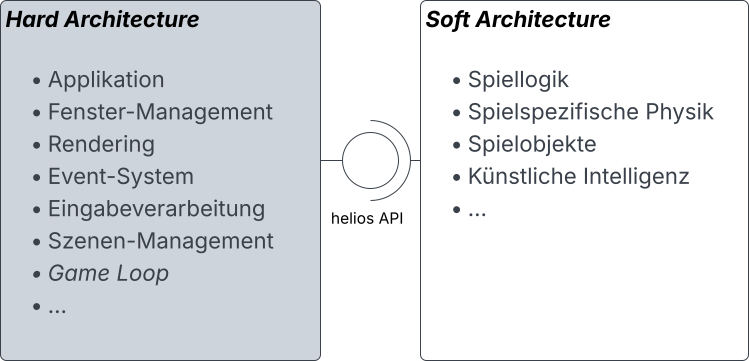
\includegraphics[width=1\columnwidth]{img/hardarchitecture.svg}
    \caption{Aufteilung der Architektur des helios Frameworks in \textit{Hard} und \textit{Soft Architecture} nach Rollings und Morris~\cite[612 ff.]{RM04}. Die Ball-/Socket-Notation verdeutlicht, dass helios Schnittstellen zur Verfügung stellt, die von einem (beliebigen) Spiel genutzt werden können. (Quelle: eigene Darstellung)}
    \label{fig:hardarchitecture}
\end{figure}

In Abbildung~\ref{fig:package_diagram} ist eine detailliertere Sicht auf die Module und ausgewählte Komponenten dargestellt.
Die Verzeichnisstruktur von helios spiegelt die Gliederung seiner Kernfunktionalitäten wider.
Im Sinne von \textit{Evans} ist dies entscheidend für eine hohe Kohäsion: Die Verzeichnisnamen kommunizieren die enthaltenen Funktionalitäten~\cite[180 f.]{Eva03}.
Innerhalb der Module findet eine weitere Unterteilung nach Schichten statt (etwa \texttt{controller}), was insgesamt als ``package-by-feature und -by-layer`` bezeichnet wird.


\begin{figure*}[t]
    \centering
    \makebox[\textwidth][c]{% Box ist textbreit, Inhalt darf überstehen
    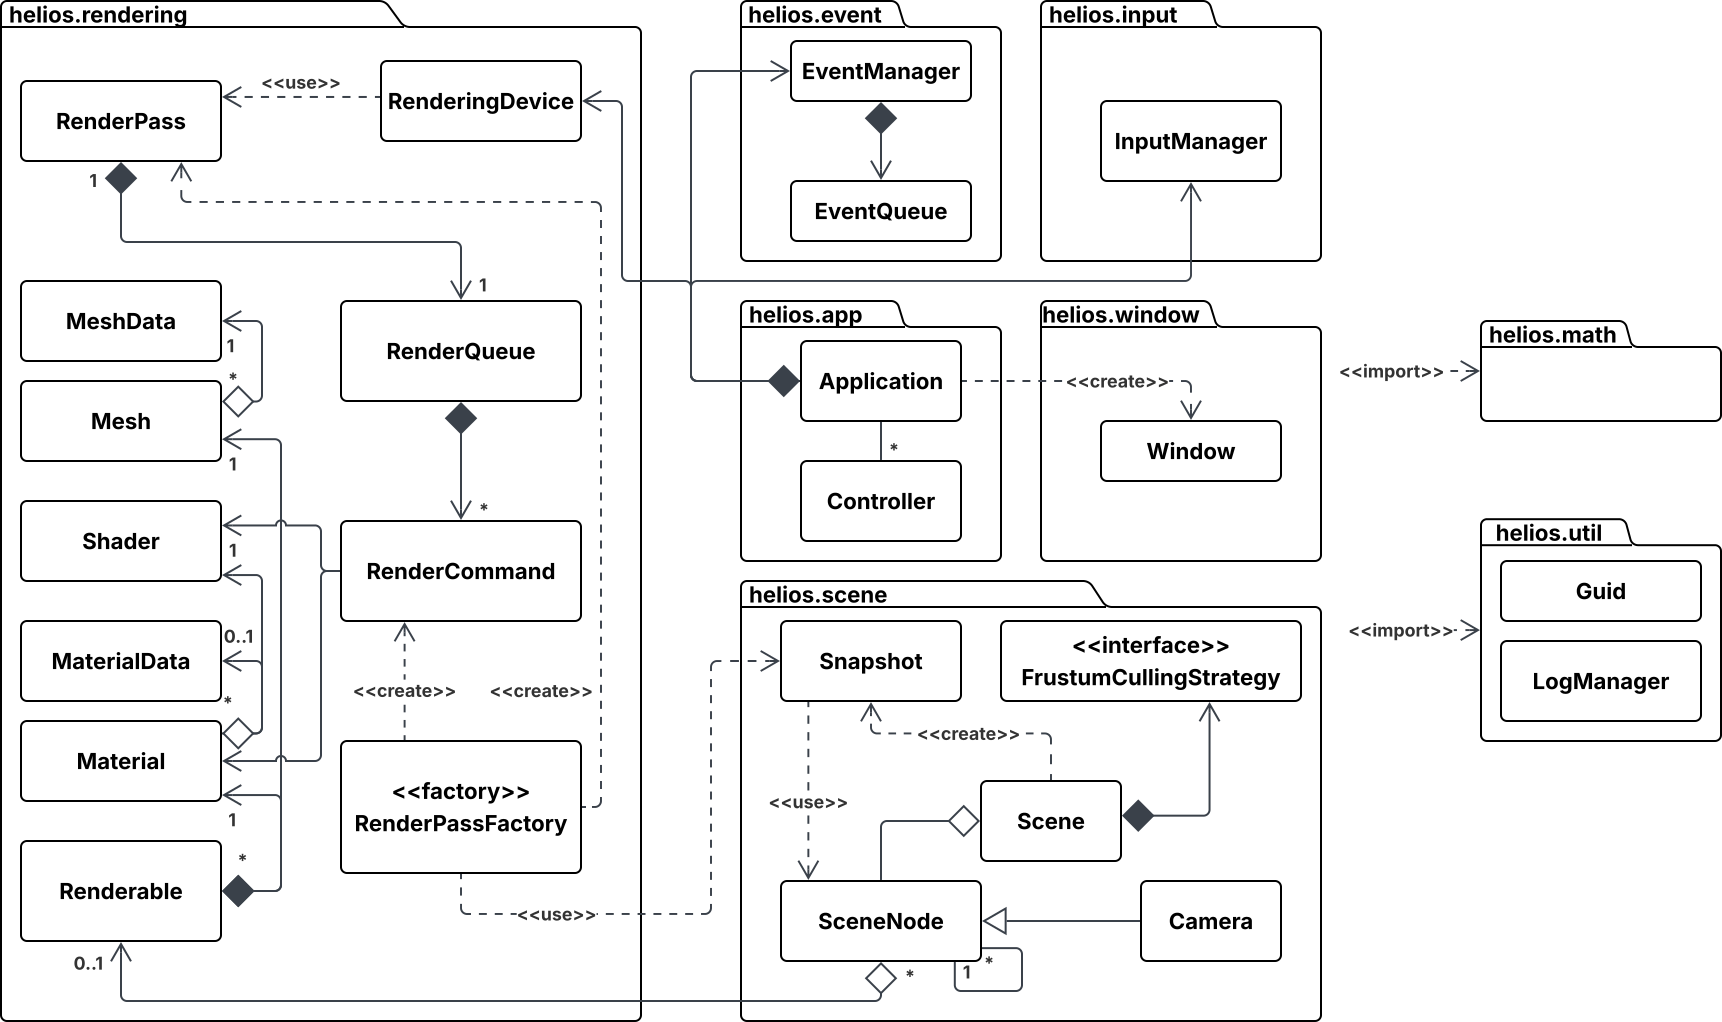
\includegraphics[width=1.4\textwidth]{img/package_diagram.svg}% \linewidth == Spaltenbreite
    }
    \caption{Aufbau des helios Framework und Zusammenhang einiger ausgewählter Komponenten. Die Strukturierung der Module orientiert sich an einem ``by-Feature, by-Layer``-Konzept, bei dem Features intern in funktionale Schichten gegliedert sind. (Quelle: eigene Darstellung)}

    \label{fig:package_diagram}

\end{figure*}


\subsection*{\texttt{app}: Applikationsschicht}
Die zentrale Steuereinheit der Anwendung bzw. des Spiels bildet die Klasse \texttt{Application}, die über Event-System, Eingabeverarbeitung und Fenstermanagement verfügt sowie das Rendering-Backend - repräsentiert durch \texttt{RenderDevice} - initialisiert.\par
helios unterstützt an dieser Stelle außerdem dynamisches Hinzufügen von Applikations-Controllern~\cite[379]{Fow03} zur Definition isolierter, ereignisbasierter Steuerungslogik, beispielsweise dem Verhalten bei einem Window-Resize\footnote{
Die Applikations-Controller wurden ursprünglich eingeführt, um ``Framebuffer-Resize``-Ereignisse gegenüber dem Rendering-Backend zu abstrahieren.
}.

\subsection*{\texttt{input}: Eingabeverarbeitung}
Der \texttt{InputManager} orchestriert die Eingabeverarbeitung.
Er wird ausschließlich von der Anwendung verwaltet und an das aktive Fenster gebunden.\par
Ein spezialisierter \texttt{InputAdapter} abstrahiert von den durch die TPLs bereitgestellten Eingabeereignissen und übersetzt sie für den \texttt{InputManager}.
Zu Beginn der Game Loop werden aktive Eingabeereignisse gepollt (\texttt{InputManager::poll()}). Eine Abfrage der Ereignisse erfolgt über Methoden wie \texttt{InputManager::isKeyPressed()}.

\subsection*{\texttt{event}: Ereignisverarbeitung}
Ereignisse können über den \texttt{EventManager} in eine \texttt{EventQueue} geschrieben werden (``\textit{post}``).
Interessierte Beobachter (\textit{Observer}) können sich über Callbacks mittels \texttt{subscribe} bei dem \texttt{EventManager} registrieren~\cite[293 ff.]{GHJV94}.
Die Methode \texttt{EventManager::dispatchAll()} informiert die Observer über vorhandene Ereignisse.

\subsection*{\texttt{window}: Fensterklasse}
Die \texttt{Window}-Klasse stellt Schnittstellen zur Steuerung des Anwendungsfensters, zur Abfrage von Fensterereignissen und zur Anweisung des \textit{Buffer-Swappings} bereit.


\subsection*{\texttt{math}: Mathematische Typen und Operationen}
Dieses Modul stellt im Namespace \texttt{helios::math} trigonometrische Funktionen und Repräsentanten für in der Linearen Algebra verankerte Datentypen wie Vektoren und Matrizen bereit.
Es unterstützt außerdem Operationen für lineare und affine Transformationen und realisiert damit den in der  3D-Computergrafik gebräuchlichen Koordinatenraumwechsel\footnote{
    Nach der Projektion liegen die Koordinaten im sogenannten \textit{Clip-Space} vor. Typischerweise sorgt das Rendering-Backend mittels perspektivischer Division dafür, dass diese Koordinaten in die für den Raterizer relevanten NDC (\textit{Normalized Device Coordinates}) umgewandelt werden~\cite[18]{AHHP+18}.
}

\[
    \text{Model}\rightarrow\text{World}\rightarrow\text{View}\rightarrow\text{Projection}
\]

\noindent

Die Schnittstellen orientieren sich bei den Methodensignaturen an populären Bibliotheken wie dem bereits erwähnten \texttt{glm}.

\subsection*{\texttt{scene}: Szenengraph}
Der Szenengraph \texttt{helios::scene::Scene} folgt etablierten Implementierungen aus der Literatur\footnote{Siehe unter anderem~\cite[]{She07} sowie~\cite[]{Gre19}.}.
\texttt{Scene} besitzt einen impliziten Wurzelknoten, der eine beliebige Anzahl von Kindknoten enthalten kann.
Jeder \texttt{SceneNode} verfügt über ein \texttt{Transform}-Objekt, das die Modelltransformation im lokalen Koordinatensystem beschreibt.\par
\texttt{SceneNodes} können ``darstellbar`` sein, das heißt, sie sind mit einem \texttt{Renderable} konfiguriert.
Sie können aber auch einfach nur eine Kamera (\texttt{helios::scene::Camera}) repräsentieren\footnote{
    Als weitere Knotentypen sind in diesem Kontext üblicherweise (frei positionierbare) \texttt{LightNodes}, also Lichtquellen, vorgesehen.
}.\par
Szenenknoten mit \texttt{Renderable} werden beim \textit{Culling} berücksichtigt.
Das Culling-Verfahren wird in der rein virtuellen Klasse \textit{FrustumCullingStrategy} abstrakt definiert. Spezialisierungen werden der \texttt{Scene} bei der Instanziierung übergeben.\par
In der Application Stage~\cite[687]{Gre19} erstellt helios aus einer Szene und einer Kamera einen \texttt{Snapshot}, für den die konfigurierte Culling-Strategie alle im sichtbaren Bereich der Kamera befindlichen \texttt{SceneNode}s sammelt.
Ein einzelner Snapshot bildet die Grundlage für einen \texttt{RenderPass}, der die nötigen Anweisungen (\texttt{RenderCommand}s) für den eigentlichen Rendering-Prozess enthält.
Listing~\ref{lst:gameloop} zeigt den Ablauf einer einfachen Game Loop.


\begin{lstlisting}[style=c++style, caption={Implementierung einer einfachen Game Loop in helios. Von der Szene wird ein \texttt{Snapshot} erstellt, der als Grundlage für den \texttt{RenderPass} dient.}, label=lst:gameloop]
while (!win->shouldClose()) {
  app->eventManager().dispatchAll();

  inputManager.poll(0.0f);

  if (inputManager.isKeyPressed(Key::ESC)) {
      win->setShouldClose(true);
  }

  snapshot   = scene->createSnapshot(*camera);
  renderPass = factory.buildRenderPass(
    snapshot
  );

  app->renderingDevice().render(renderPass);

  win->swapBuffers();
}
\end{lstlisting}



\subsection*{\texttt{rendering}: Render Pipeline}
Das Rendering-System von helios ist in verschiedene Module aufgeteilt, darunter \texttt{shader} für Shader- und GLSL\footnote{\textit{OpenGL Shading Language}}-spezifischen Code sowie \texttt{model} für Abstraktionen von Material- und Mesh-Daten.\par
\texttt{Renderable}s sind Repräsentanten ``darstellbarer`` Objekte.
Sie kapseln für den Rendering-Prozess notwendige Informationen und sind als Aggregation modelliert.
Sie bestehen aus individuell konfigurierbaren \texttt{Material}- und \texttt{Mesh}-Instanzen, die wiederum \texttt{MaterialData}- und \texttt{MeshData}-Objekte zur einfachen und ressourcenschonenden Wiederverwendung mit anderen Instanzen teilen~\cite[126]{AHHP+18}.\par

Die für einen \texttt{RenderPass} benötigten Informationen werden als \texttt{RenderCommand}-Objekte in einer \texttt{RenderQueue} gesammelt, die vom eigentlichen \texttt{RenderDevice} verarbeitet werden: \texttt{RenderCommand}s besitzen Zeiger auf die darzustellende Geometrie (\texttt{Mesh}), die zu nutzenden \texttt{Shader} sowie Daten-Objekte, in denen Informationen zu \texttt{Uniform}-Variablen (Transformationsmatrizen etc.) gespeichert sind.\par
Das \texttt{RenderDevice} verarbeitet einen \texttt{RenderPass} über Template-Methoden \texttt{preRender, doRender} und \texttt{postRender}.


\subsection*{\texttt{util}: Utility-Klassen}
Im Modul \texttt{helios::util} liegt nicht-domänenspezifischer Code, wie der \texttt{LogManager} für einfache Logging-Funktionalitäten sowie eine \texttt{Guid}-Implementierung zur Konfiguration von Objekten mit einem globalen eindeutigen Identifikator (\textit{global unique identifier}).
\section{Diskussion der Umsetzung}

Petrillo et al. beschreiben in~\cite[]{PPTD08} mehrere Ursachen, die zu \textit{Feature Creep} in der Spieleentwicklung führen.
Dazu zählen unter anderem die Entwicklung eigener Lösungen anstelle der Nutzung bestehender Bibliotheken, sowie das Hinzufügen vermeintlich ``attraktiver`` Features, die unter Berücksichtigung der \textit{YAGNI}\footnote{\textit{You Aren't Gonna Need It}~\cite[]{Sch07}}-Maxime keinen Mehrwert für das eigentliche Projektziel bieten.
Damit steht die Spielentwicklung, wie die Autoren hervorheben, auf gleicher Stufe mit der ``gewöhnlichen`` Softwareentwicklung, etwa im Rahmen von Auftragsarbeiten.
Handelt es sich zudem um ein Projekt mit einer fachlich unbekannten Domäne, das in einem engen Zeitrahmen umgesetzt werden muss, sind Augenmaß und Disziplin bei der Realisierung von Funktionalität unerlässlich.
Mit helios verfolgen wir daher einen Top-Down-Ansatz, um ein schnelles Prototyping zu ermöglichen und unter Anwendung des Framework-Gedankens die schrittweise Entwicklung und Integration des \textit{Geometry Wars}-Klons voranzutreiben.
In diesem Zusammenhang verstehen wir die SOLID\footnote{
\textbf{S}ingle-Responsibility-Prinzip, \textbf{O}pen-Closed-Prinzip, \textbf{L}iskovsches Substitutionsprinzip, \textbf{I}nterface-Segregation-Prinzip, \textbf{D}ependency-Inversion-Prinzip
}-Prinzipien~\cite[]{Mar03} als unverzichtbare Basis agiler Softwareentwicklung, da sie in engem Zusammenhang mit einem ``sauberen Softwaredesign`` stehen und sich im bisherigen Entwicklungsprozess bereits als wertvoll erwiesen haben\footnote{Vgl. Cabral et al., die in~\cite[]{CKME+24} SOLID im Machine-Learning-Umfeld untersuchen - einem Umfeld, das von ``iterativen Experimenten mit Daten, Modellen und Algorithmen`` (eigene Übersetzung) geprägt ist. Sie kommen zu dem Schluss, dass die Anwendung der Prinzipien wesentlich zum Quellcodeverständnis beiträgt.}.

Um die Entstehung einer unstrukturierten, schwer wartbaren Architektur (\textit{Big Ball of Mud}~\cite[]{FY99}) zu vermeiden, setzen wir auf eine klare Trennung der Verantwortlichkeiten, die sich in dem Projekt durch die verschiedenen Feature-Layer widerspiegelt.
Zur Reduktion des Kopplungsgrads zwischen beteiligten Komponenten - und somit zur Verbesserung von Wartbarkeit und Testbarkeit - nutzen wir \textit{Dependency Injection}~\cite[]{SZ10}, was überwiegend durch \textit{Constructor Injection}~\cite[]{FowlerDI} realisiert wird.
Da in der aktuellen Implementierung kein dedizierter DI-Container zur Anwendung kommt, entsteht durch die Verwaltung der Abhängigkeiten (``\textit{wiring}``) im eigentlichen Quelltext zusätzlicher Boilerplate-Code, der jedoch weitgehend durch die Auslagerung von Erzeugungslogik in statische Factory-Klassen reduziert wird.
Davon profitieren gerade die Implementierungen der Beispielprogramme während der Entwicklung, die auch als Testprogramme dienen.
In anderen Subsystemen unterstützen darüber hinaus Factory-Methoden die Kapselung der Objekterzeugung innerhalb jener Entitäten, denen auch fachliche Verantwortlichkeit im Sinne der Geschäftslogik zugeordnet ist~\cite[139 f.]{Eva03}.
Auf diese Weise bleibt die Architektur von helios kohärent, und Abhängigkeiten zwischen den Schichten sind auf das notwendige Minimum beschränkt.


Als eher herausfordernd empfinden wir den Umgang mit modernen Sprachfeatures, die eine bewährte, aber auch ``traditionelle`` Programmiersprache wie C++ in den letzten Jahren erfahren hat - etwa das Modulsystem oder den Einsatz von Smart-Pointern: Dabei sehen wir uns im Spannungsfeld, etablierte C++-Idiome~\cite[]{IdiomaticCpp} und bewährte Konzepte in einer Entwicklungsumgebung anzuwenden, die überwiegend von Erfahrungen aus einfacheren Hochsprachen wie Java geprägt ist.
Gerade zu Beginn des Projekts wurde die Projektstruktur sowie Bezeichner von Namensräumen deshalb immer wieder angepasst (siehe Abbildung~\ref{fig:code_frequency}).

\begin{figure}[!h]
    \centering
    \includegraphics[width=0.8\columnwidth]{img/code_frequency}
    \caption{Code-Frequenz Graph für das helios-Repository. Die in der Frühphase erfolgten Änderungen an der Projektstruktur spiegeln sich in der nahezu symmetrischen Verteilung von hinzugefügtem (grün) und entferntem Code (rot) wider. (Quelle: GitHub)}
    \label{fig:code_frequency}
\end{figure}

Um bei der Objektverwaltung klare Besitzverhältnisse auszudrücken, verzichten wir an vielen Stellen auf \textit{raw pointer}.
Stattdessen greifen wir auf die in der Standardbibliothek definierten \texttt{unique\_ptr}, \texttt{shared\_ptr} oder \texttt{weak\_ptr}-Typen zurück, die Besitzsemantiken exklusiv (durch \textit{move}-Operationen) oder gemeinsam (durch Referenzzählung) verwalten.
Inwieweit die hierdurch entstehenden zusätzlichen CPU-Instruktionen\footnote{Einen Performance-Vergleich bietet beispielsweise~\cite[]{Val25}} beim Aufbau und der Bearbeitung der Rendering-Pipeline messbare Auswirkungen auf die Effizienz haben, muss gegebenenfalls zu einem späteren Zeitpunkt evaluiert werden.

Wir sehen hierin ein mögliches Optimierungspotenzial, entscheiden uns in der frühen Entwicklungsphase jedoch bewusst für Stabilität und klare Semantik.
Spätere  Refactorings zugunsten einer höheren Effizienz\footnote{
Diese beschränken sich nicht unbedingt auf das Design der Komponenten oder die Architektur selbst, sondern können sich bis auf niedrige Abstraktionsebenen erstrecken - etwa ``bare metal`` hin zu Implementierungen der Mathebibliothek mittels SIMD-Instruktionen, wie sie von \texttt{glm}~\cite[]{glmSimd} bereitgestellt wird. SIMD, als Abkürzung für \textit{single instruction, multiple data}, beschreibt das Konzept, bei dem eine einzelne Instruktion parallel auf unterschiedliche Daten ausgeführt wird.
} nehmen wir also in Kauf, zumal solche Maßnahmen ohnehin erst dann sinnvoll scheinen, wenn die Domäne sowohl fachlich als auch technisch hinreichend durchdrungen ist\footnote{
   Siehe ``Refactoring toward Deeper Insight``~\cite[]{Eva03}.
}.


Nicht unerwähnt bleiben soll an dieser Stelle die Wahl der Datenstrukturen und der Programmierparadigmen: Unsere Objektbeziehungen sind derzeit sehr ausdrucksstark (\texttt{Snapshot}, \texttt{Renderable}, \texttt{Material}, \texttt{Shader}, usw.), übermäßig tiefe Vererbungshierarchien haben wir bislang vermeiden können.
Die Entscheidung, Vektoren als primäre Datencontainer zu verwenden, kann sich potenziell negativ auf die Rendering-Pipeline auswirken, wenn die Render-Queue nach einer Aktualisierung der Szene neu aufgebaut und dabei zusätzlicher Speicher zur Laufzeit alloziiert werden muss.

Weitere Optimierungspotenziale sehen wir im Design des \texttt{EventManagers} und der Eingabeverarbeitung: Beide Systeme können zusammengeführt werden, sodass auch Eingabebefehle nach dem Prinzip ``Don't call us, we call you`` als Ereignisse an interessierte Beobachter weitergeleitet werden.
Dabei ist zu berücksichtigen, dass dem Spiel hierzu Schnittstellen zur Verfügung gestellt werden müssen und eine Bottom-up Kommunikation erlaubt sein muss~\cite[]{BMRS+96}.
Darüber hinaus soll eine Mechanik geschaffen werden, die aus Eingabeereignissen spielspezifische \texttt{ControlCommand}s ableitet~\cite[21 ff.]{Nys14}.

Bei der Architektur des Rendering-Systems sehen wir eine Grundlage für eine modulare und erweiterbare Rendering-Pipeline, die derzeit eine klare Trennung zwischen Szenenbeschreibung und eigentlichem Rendering realisiert.
Der Vorteil des gewählten Designs liegt darin, dass die individuellen \texttt{RenderPass}-Instanzen mit zusätzlichen Optionen konfiguriert werden können (beispielsweise \textit{Depth Testing}, \textit{Draw Mode}, \textit{Anti-Aliasing} u.a.) und die \texttt{RenderQueue}s so sortiert werden können, dass die Kommunikation mit der GPU möglichst effizient stattfinden kann\footnote{
    Unity~\cite[]{UnityRenderQueue} und OGRE~\cite[]{OgreRenderQueue} verfolgen ähnliche Konzepte; auch Diskussionen von Christer Ericson~\cite[]{ChristerEricson} thematisieren die Sortierung des Render-Pass. Vulkan bietet explizite Render-Pass-Semantik~\cite[]{VulkanRenderPass}
}.
Ob sich das Design im Rahmen der Implementierung des eigentlichen Spiels bewährt - und diese Features überhaupt benötigt werden - wird sich in der weiteren Entwicklung zeigen.




\section{Abschluss und Ausblick}

Wir haben \textit{helios} vorgestellt, einen Prototypen für ein Game Framework zur Umsetzung eines \textit{Geometry Wars}-Klon.

Es folgte ein Überblick über die Projektdaten sowie über Aufbau und Architektur des C++-Projekts.
Dabei sind wir auf die Toolchain eingegangen und haben die verwendeten Bibliotheken von Drittanbietern vorgestellt.\\

Schwierigkeiten bei der Umsetzung haben wir in einer Diskussion reflektiert.
Aus diesen Reflexionen haben sich für uns interessante Fragen ergeben, die einer näheren Betrachtung wert sind:
Wie wirken sich verschiedene Formen der Game Loop~\cite[534 ff.]{Gre19} auf das \textit{Game Feel} aus?
Welchen Einfluss auf die Laufzeit haben die aus der Standardbibliothek übernommenen Datenstrukturen bei Neuallokation im \textit{Hot Path} des Renderings?
Und welchen Performancevorteil würden wir durch den Einsatz von \textit{raw pointern} im Gegensatz zu \textit{Smart Pointern} erzielen?\\

Aufgrund der konsequenten Anwendung allgemein anerkannter Entwicklungsprinzipien sehen wir derzeit wenig Bedarf an strukturellen Änderungen.
Es empfiehlt sich jedoch, hier keine voreiligen Schlüsse zu ziehen:
Bevor die technische Domäne vollständig durchdrungen ist, steht noch eine fachliche Auseinandersetzung mit den intrinsischen Eigenschaften von Kollisionsbehandlungsstrategien sowie (künstlicher) Gegnerintelligenz an.
Hier erwarten wir mehrere weitere Entwicklungsschleifen.
Im gleichen Zusammenhang betrachten wir auch den Entwurf der Rendering-Pipeline vorsichtig optimistisch.
Zwar folgt dieser klaren semantischen Strukturen und orientiert sich am \textit{mental model} eines Entwicklers.
Unsere Recherche hat jedoch gezeigt, dass datengetriebene Entwicklung~\cite{Bay22} und hardwarenahe Optimierungen durchaus zum Usus effizienter Spiele gehören.\\

Bei alldem soll nicht vergessen werden, dass wir in dieser frühen Phase des Projekts bewusst eine robuste Implementierung bevorzugt haben.
Wir blicken den nachfolgenden Iterationen daher gespannt entgegen.
Mit dem Projektziel ``16 ms pro Frame`` vor Augen schließen wir diesen Abschnitt mit einem Zitat von Donald E. Knuth:
\begin{quote}
    \centering
    \textit{``Premature optimization is the root of all evil.``}~\cite{Knu74}
\end{quote}

\input{content/de/8. danksagung}
\clearpage
\appendix
\section{Veröffentlichungshinweis}

Dieses Dokument wurde im Rahmen der Projektarbeit im Fernstudiengang Informatik an der Trier University of Applied Sciences erstellt.
Es dokumentiert den ersten Meilenstein des Projekts \textit{helios}, einem C++-basierten Framework-Prototypen zur Entwicklung eines \textit{Geometry Wars}-ähnlichen Spiels.\\

\noindent
\subsection*{Urheberrecht \& Lizenz}
\textcopyright 2025 Thorsten Suckow-Homberg.\\
Dieses Werk steht unter der Creative Commons Namensnennung 4.0 International Lizenz (CC BY 4.0).
Die vollständige Lizenz ist unter \url{https://creativecommons.org/licenses/by/4.0/} abrufbar.


\subsection*{Hinweis zu Markennamen}\\
\textit{Geometry Wars} ist ein eingetragenes Markenzeichen von Activision Publishing, Inc.
Das in diesem Bericht beschriebene Projekt steht in keiner Verbindung zum Originalspiel oder dessen Rechteinhabern.



%%%%%%%%%%%%%%%%%%%%%%%%%%%%%%%%%%
    \clearpage
    \sloppy
    \printbibliography
    \fussy


\end{document}
